%=========================================================
\chapter{Modelo Estatico}	

En el diseño de sistemas de software, el enfoque modular es esencial para crear aplicaciones eficientes, mantenibles y escalables. El diseño de módulos se basa en la división del sistema en componentes más pequeños y autónomos, conocidos como módulos, que encapsulan funcionalidades específicas y se comunican entre sí de manera coherente. En el contexto del sistema de la guardería "Burbujas", el diseño de módulos desempeña un papel crucial en la organización y la implementación de las diversas características y procesos que son necesarios para su funcionamiento.

El objetivo del diseño de módulos en el sistema de la "Guardería burbujas" es garantizar una estructura clara y modular, donde cada módulo se encargue de una funcionalidad específica y pueda ser desarrollado, probado y mantenido de forma independiente. Esto permite una mayor flexibilidad en el desarrollo y facilita la colaboración entre el equipo de desarrollo. Además, el diseño de módulos promueve la reutilización de código, ya que los módulos pueden ser utilizados en diferentes partes del sistema o en proyectos futuros.
\\

Al diseñar los módulos del sistema de la "Guardería burbujas", se deben tener en cuenta diferentes aspectos, como la cohesión, la modularidad y la interoperabilidad. La cohesión se refiere a la medida en que los elementos dentro de un módulo están relacionados y trabajan juntos para cumplir una funcionalidad específica. Una alta cohesión indica que un módulo tiene una única responsabilidad y se centra en una tarea concreta. Por otro lado, la modularidad se refiere a la capacidad de un módulo de ser independiente y reemplazable sin afectar el funcionamiento de otros módulos. La interoperabilidad implica que los módulos deben poder comunicarse entre sí de manera eficiente y consistente, a través de interfaces bien definidas y protocolos de interacción.

%-----------------------------------------------------------------------
\section{Diseño de Subsistemas}

En el diseño de sistemas complejos, como es el caso del sistema de la guardería "Guardería Burbujas", se utiliza el concepto de subsistemas para organizar y estructurar las diferentes partes o componentes del sistema. Un subsistema es una unidad funcionalmente independiente dentro de un sistema más grande, que tiene la capacidad de realizar tareas específicas y contribuir al funcionamiento global del sistema.

Los subsistemas se utilizan para dividir un sistema en componentes más pequeños y manejables, lo cual facilita el diseño, la implementación y el mantenimiento del sistema en su conjunto. Cada subsistema tiene su propia funcionalidad y responsabilidades, y puede interactuar con otros subsistemas para lograr los objetivos del sistema en su conjunto.

El diseño de subsistemas implica identificar las diferentes partes o módulos del sistema que pueden funcionar de manera independiente pero también interactuar entre sí. Cada subsistema puede tener su propia arquitectura interna, sus interfaces con otros subsistemas y sus propias reglas y lógica de funcionamiento.

El diseño de subsistemas se basa en el principio de modularidad, que consiste en dividir un sistema en componentes más pequeños y cohesivos. Cada subsistema se enfoca en una funcionalidad específica y puede ser desarrollado y probado de manera independiente. Esto permite un desarrollo paralelo y una mayor reutilización de componentes en futuros proyectos.

En el contexto del sistema de la guardería "Guardería Burbujas", se pueden identificar varios subsistemas, como el subsistema de Gestion infantes, el subsistema de Gestión de padres de familia, el subsistema Gestión de días hábiles, el subsistema de Gestión de personal, el subsistema de Gestión de clases y el subsitema de Salud

\begin{figure}[htbp]
	\begin{center}
		\fbox{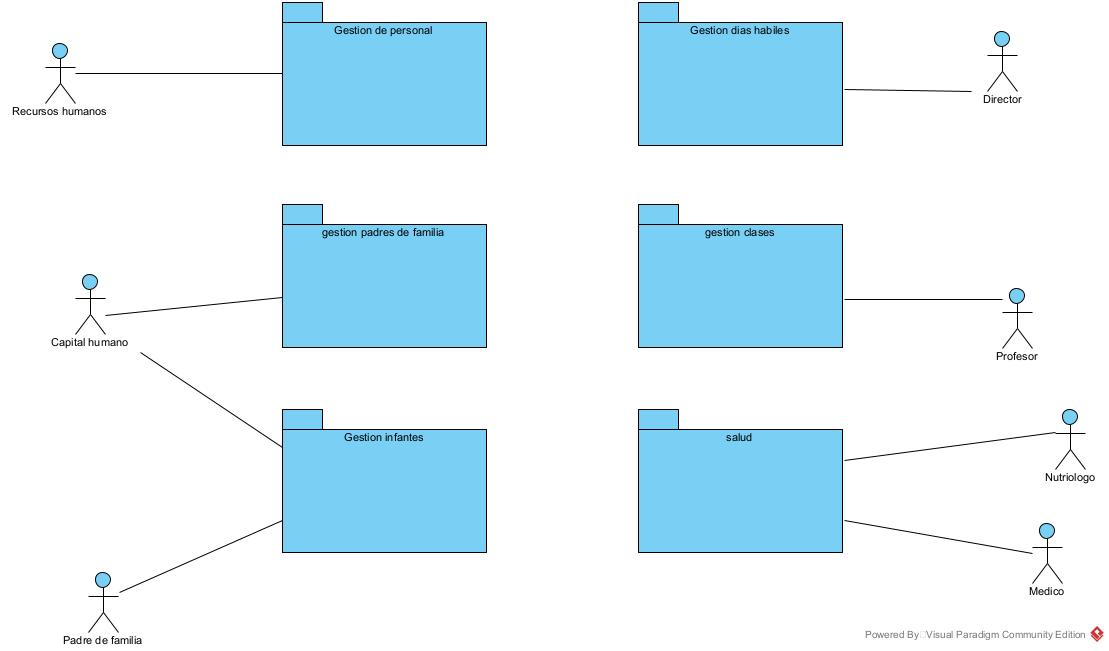
\includegraphics[width=.8\textwidth]{images/casosDeUso}}
		\caption{Diagrama de casos de uso del sistema.}
		\label{fig:casosDeUso}
	\end{center}
\end{figure}

Que son los subsitemas para los actores Recursos Humanos, Capital humano, Padre de familia, Médico, Nutriólogo, Director y Profesor.

\clearpage
%------------------------------------------------------------------
\subsection{Subsistema de Gestión de personal}
El personal de la guardería es un elemento clave para brindar un ambiente seguro, cuidadoso y estimulante para los niños. El subsistema de Gestión de Personal tiene como objetivo garantizar que se cuente con un equipo de profesionales capacitados y comprometidos, que cumplan con los requisitos de calificación necesarios y estén disponibles en los momentos adecuados para brindar atención y cuidado a los infantes.
\\
Este subsistema involucra diferentes actores, como el Director de la guardería, los Recursos Humanos y los propios miembros del personal. Cada actor desempeña un papel específico en la gestión del personal, desde la contratación y el proceso de selección hasta la asignación de tareas y la supervisión del rendimiento.

\begin{figure}[htbp]
\centering
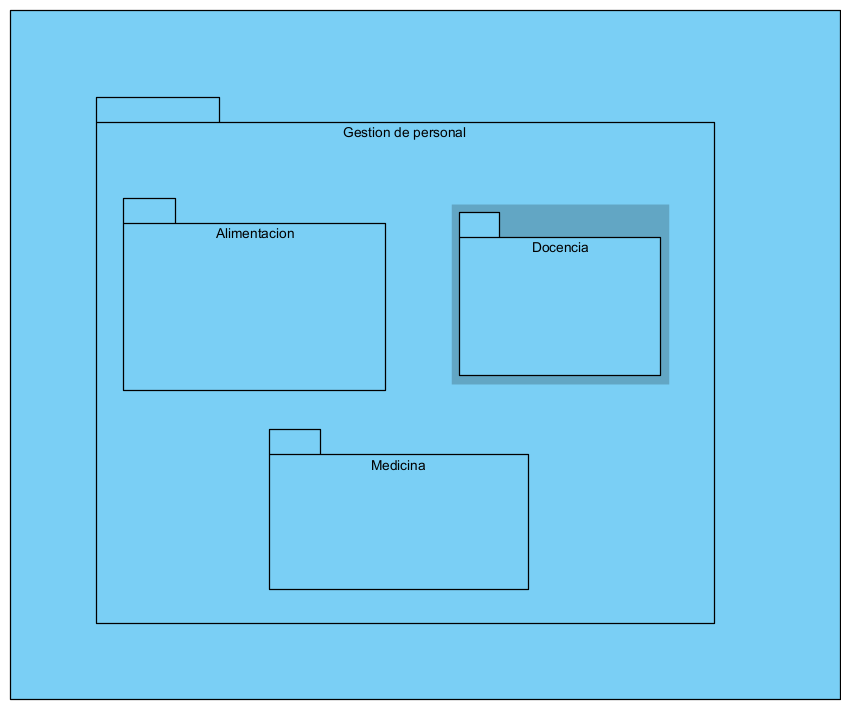
\includegraphics[width=0.7\textwidth]{images/arqui/subPersonal.png}
\caption{Subsistema Gestion de personal.}
\label{fig:subsistsalud}
\end{figure}

\subsubsection{Submódulo de Docencia}
El modulo "Docencia" es una parte integral del sistema de la guardería "Guardería Burbujas" y se encarga de gestionar todos los aspectos relacionados con el personal docente. Este módulo permite llevar un control eficiente del cuerpo docente, garantizando una educación de calidad y un entorno de aprendizaje óptimo para los niños.

El módulo de Docencia ofrece las siguientes funcionalidades:

\begin{itemize}
\item[*] Registro de profesor: Esta funcionalidad permite ingresar y almacenar la información relevante de los profesores que formarán parte del equipo docente de la guardería. Se recopilan datos como el nombre, la experiencia educativa, las especialidades y cualquier otra información necesaria para la asignación adecuada de los profesores a los grupos de niños.
\item[*] Dar de baja a profesor: En caso de que sea necesario, esta funcionalidad permite dar de baja a un profesor del sistema. Esto puede ocurrir por diversos motivos, como cambios en el personal, finalización de contrato o cualquier otra circunstancia que requiera la eliminación de un profesor del registro del sistema. Al dar de baja a un profesor, se actualiza la información de disponibilidad del personal docente.
\item[*] Actualización de datos del profesor: Esta funcionalidad permite realizar modificaciones y actualizaciones en la información de los profesores registrados. Puede incluir cambios en la información de contacto, actualización de experiencia educativa, incorporación de nuevas especialidades o cualquier otro dato relevante para mantener los registros del profesorado al día.
\end{itemize}

El módulo de Docencia es esencial para garantizar que el personal docente esté adecuadamente registrado, actualizado y asignado a los grupos de niños correspondientes. Esto facilita la planificación y organización de las clases, asegurando una distribución equitativa de los profesores y una atención de calidad en el proceso educativo de los infantes.

\begin{figure}[htbp]
\centering
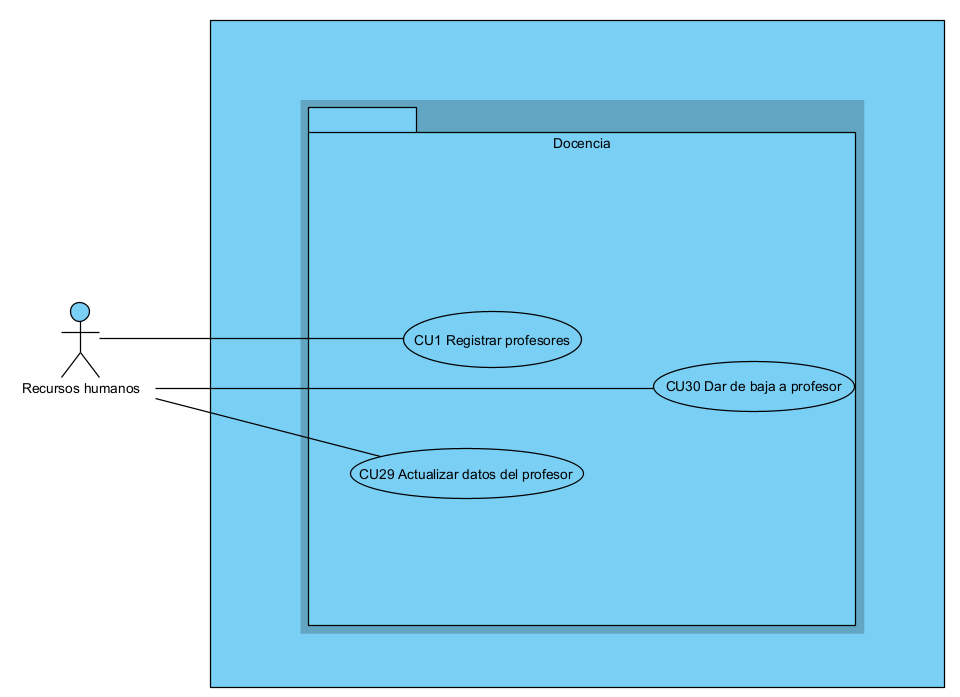
\includegraphics[width=0.7\textwidth]{images/arqui/subConsulDoce.png}
\caption{Modulo de Docencia del subsistema Gestion de personal.}
\label{fig:subsistGestDoce}
\end{figure}


\subsubsection{Submódulo de Alimentacion}

El módulo "Alimentacion" es una parte integral del sistema de la guardería "Guardería Burbujas" y se encarga de gestionar todos los aspectos relacionados con el personal de nutrición y alimentación. Este módulo permite llevar un control eficiente de los nutriólogos, asegurando una alimentación adecuada y equilibrada para los niños.

El módulo de Nutriólogo ofrece las siguientes funcionalidades:

\begin{itemize}
\item[*] Registro de nutriólogo: Esta funcionalidad permite ingresar y almacenar la información relevante de los nutriólogos que formarán parte del equipo encargado de la alimentación en la guardería. Se recopilan datos como el nombre, la experiencia en nutrición, las especialidades y cualquier otra información necesaria para la asignación adecuada de los nutriólogos a los grupos de niños.
\item[*] Dar de baja a nutriólogo: En caso de que sea necesario, esta funcionalidad permite dar de baja a un nutriólogo del sistema. Esto puede ocurrir por diversos motivos, como cambios en el personal, finalización de contrato o cualquier otra circunstancia que requiera la eliminación de un nutriólogo del registro del sistema. Al dar de baja a un nutriólogo, se actualiza la información de disponibilidad del personal de nutrición.
\item[*] Actualización de datos del nutriólogo: Esta funcionalidad permite realizar modificaciones y actualizaciones en la información de los nutriólogos registrados. Puede incluir cambios en la información de contacto, actualización de experiencia en nutrición, incorporación de nuevas especialidades o cualquier otro dato relevante para mantener los registros del personal de nutrición al día.
\end{itemize}


\begin{figure}[htbp]
\centering
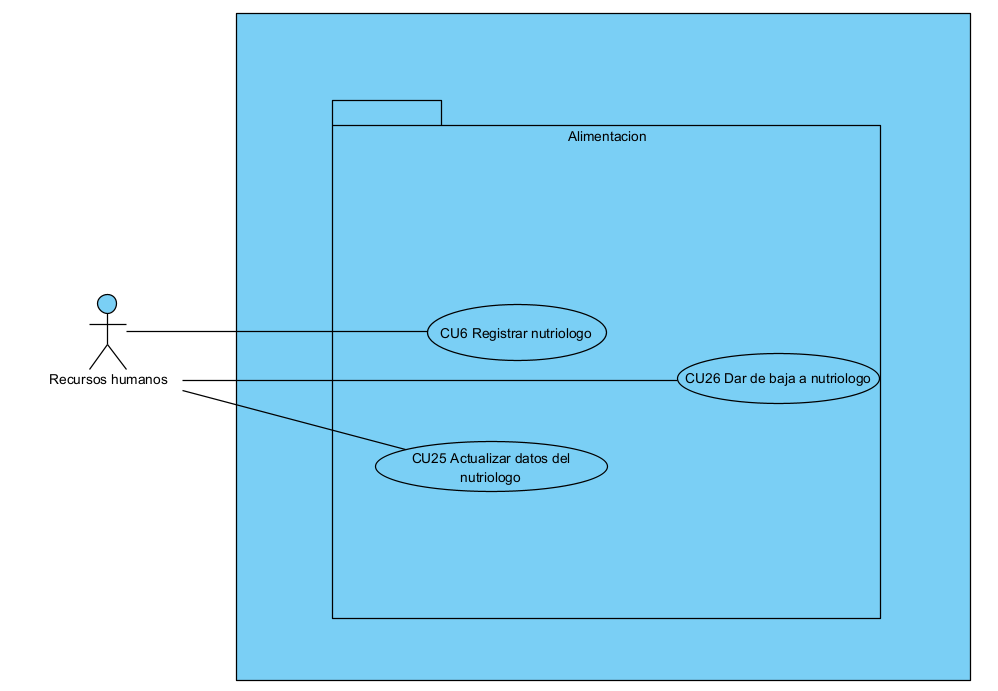
\includegraphics[width=0.7\textwidth]{images/arqui/subConsulAlimentac.png}
\caption{Modulo de Alimentacion del subsistema Gestion de personal.}
\label{fig:subsistGestalim}
\end{figure}


\subsubsection{Submódulo de Medicina}

El módulo "Medicina" es una parte integral del sistema de la guardería "Guardería Burbujas" y se encarga de gestionar todos los aspectos relacionados con el personal médico. Este módulo permite llevar un control eficiente de los médicos, asegurando la salud y el bienestar de los niños.

El módulo de Medicina ofrece las siguientes funcionalidades:

\begin{itemize}
\item[*] Registro de médico: Esta funcionalidad permite ingresar y almacenar la información relevante de los médicos que formarán parte del equipo médico de la guardería. Se recopilan datos como el nombre, la especialidad médica, la experiencia y cualquier otra información necesaria para la asignación adecuada de los médicos en el cuidado de los niños.
\item[*] Dar de baja a médico: En caso de que sea necesario, esta funcionalidad permite dar de baja a un médico del sistema. Esto puede ocurrir por diversos motivos, como cambios en el personal, finalización de contrato o cualquier otra circunstancia que requiera la eliminación de un médico del registro del sistema. Al dar de baja a un médico, se actualiza la información de disponibilidad del personal médico.
\item[*] Actualización de datos del médico: Esta funcionalidad permite realizar modificaciones y actualizaciones en la información de los médicos registrados. Puede incluir cambios en la información de contacto, actualización de especialidades médicas, incorporación de nuevas certificaciones o cualquier otro dato relevante para mantener los registros del personal médico al día.
\end{itemize}

El módulo de Medicina es esencial para garantizar que el personal médico esté adecuadamente registrado, actualizado y asignado a las tareas correspondientes. Esto facilita la atención médica de los niños, asegurando que reciban la atención adecuada en caso de enfermedades, lesiones u otras situaciones médicas que puedan surgir.


\begin{figure}[htbp]
\centering
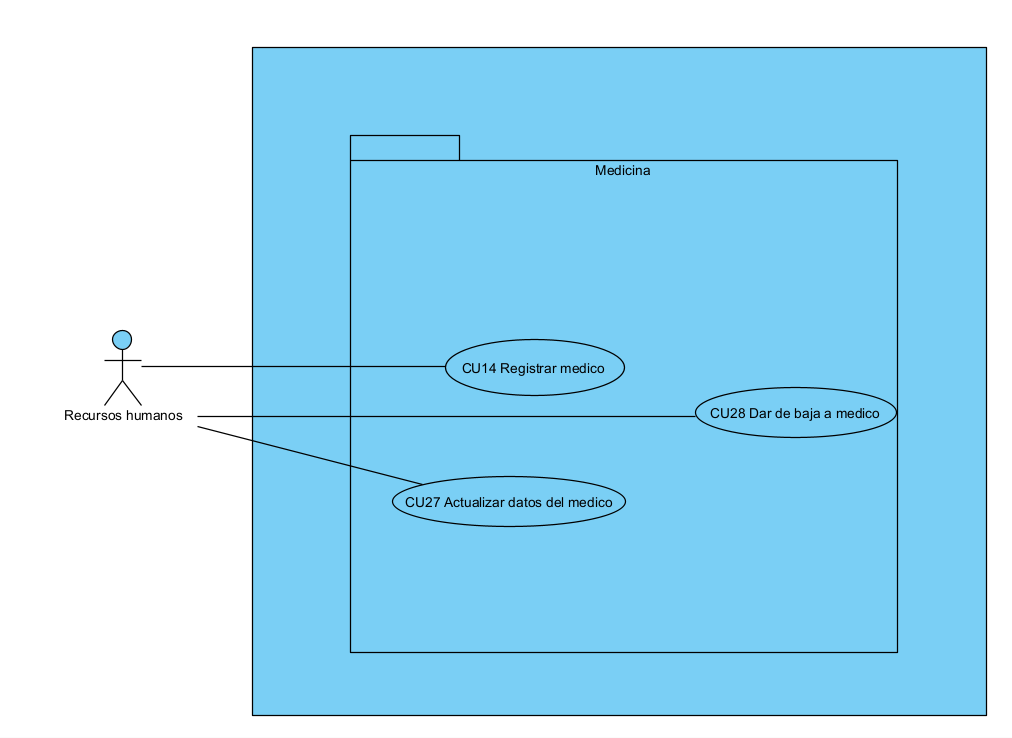
\includegraphics[width=0.7\textwidth]{images/arqui/subConsulMedicina.png}
\caption{Modulo de Medicina del subsistema Gestion de personal.}
\label{fig:subsistMedic}
\end{figure}

\clearpage
%------------------------------------------------------------------
\subsection{Subsistema de Gestión padres de familia}
El subsistema de "Gestión de padres de familia" es una parte esencial del sistema de la guardería "Guardería Burbujas". Este subsistema se encarga de administrar y mantener actualizada la información de los padres de familia de los infantes que asisten a la guardería. Su objetivo principal es tener la informacion de todos los padres de familia registrados para brindarles información relevante sobre sus hijos y garantizar una participación activa en el cuidado y desarrollo de los niños.

\begin{figure}[htbp]
\centering
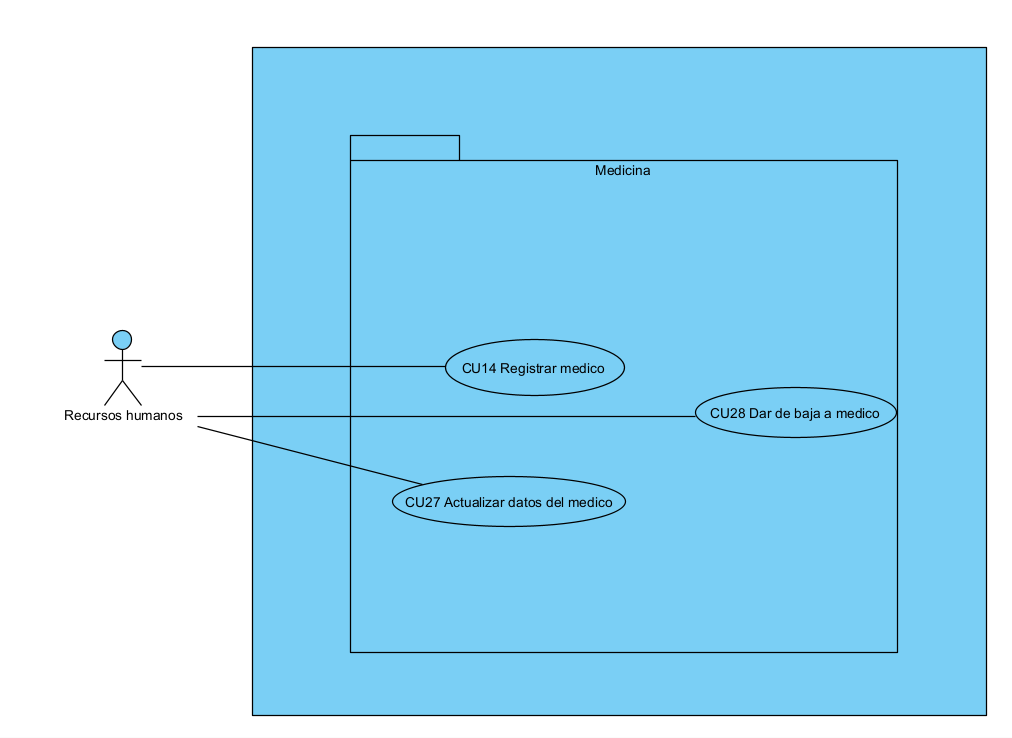
\includegraphics[width=0.7\textwidth]{images/arqui/subConsulMedicina.png}
\caption{Subsistema Gestion padres de familia.}
\label{fig:subsistGestionpapa}
\end{figure}
\clearpage
%------------------------------------------------------------------
\subsection{Subsistema de Gestión infantes}

El subsistema de "Gestión de infantes" es una parte fundamental del sistema de la guardería "Guardería Burbujas". Este subsistema se encarga de administrar y mantener actualizada la información de los infantes que asisten a la guardería, así como de supervisar su bienestar, progreso y desarrollo durante su estancia en el centro.


\begin{figure}[htbp]
\centering
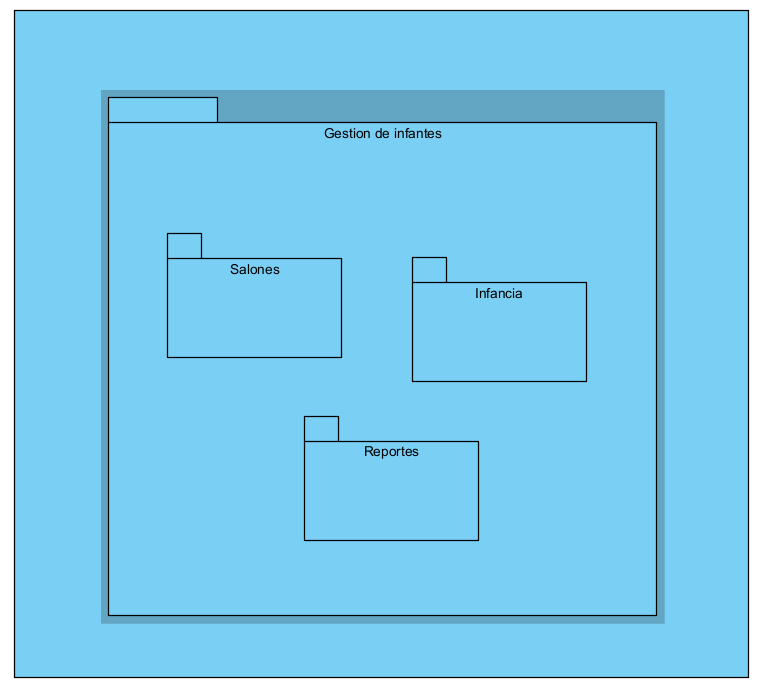
\includegraphics[width=0.7\textwidth]{images/arqui/subSisGestInfant.png}
\caption{Subsistema Gestion infantes.}
\label{fig:subsistGestionInfan}
\end{figure}

El subsistema de Gestión de infantes se divide en varios submódulos, que son los siguientes:

\subsubsection{Submódulo de salones}
El submódulo de salones tiene como objetivo principal organizar y administrar los diferentes salones de la guardería. En este submódulo se gestionan aspectos como la asignación de infantes a los salones correspondientes, la distribución equitativa de niños por grupo de edad y la supervisión de la capacidad máxima de cada salón. Además, se registran y actualizan datos relevantes de cada salón, como el nombre, la ubicación, los horarios y las actividades programadas.


\begin{figure}[htbp]
\centering
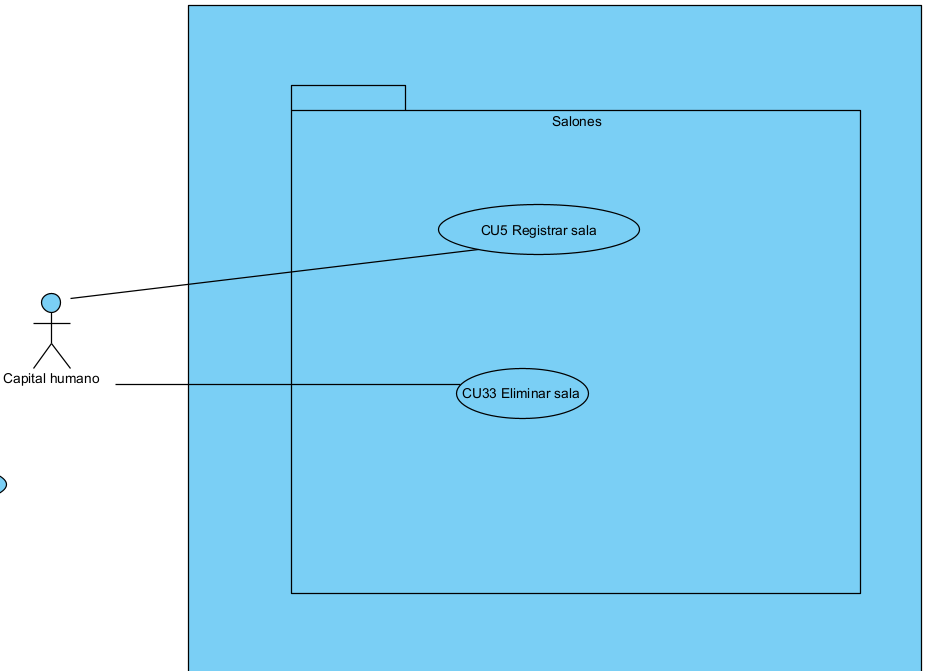
\includegraphics[width=0.7\textwidth]{images/arqui/subSisGestInfantSalon.png}
\caption{Diagrama del Submodulo de salones.}
\label{fig:subsistGestionInfansalones}
\end{figure}

\subsubsection{Submódulo de infancia}
El submódulo de infancia se encarga de recopilar y mantener actualizada la información personal y médica de cada infante. En este submódulo se registran datos como el nombre, la fecha de nacimiento, los contactos de emergencia, las alergias, las enfermedades crónicas y cualquier otra información relevante para brindar una atención adecuada y personalizada a cada niño. Además, se realiza un seguimiento del desarrollo y los hitos alcanzados por cada infante, lo que permite detectar y abordar oportunamente cualquier necesidad o preocupación.

\begin{figure}[htbp]
\centering
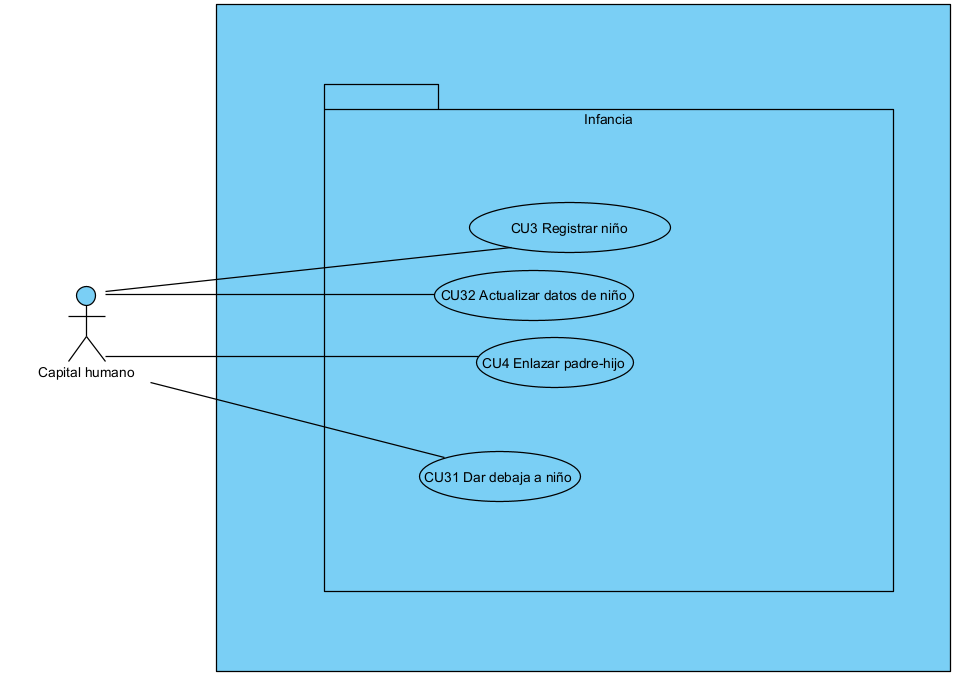
\includegraphics[width=0.7\textwidth]{images/arqui/subSisGestInfantInfancia.png}
\caption{Diagrama del Submodulo de infancia.}
\label{fig:subsistGestionInfanInfancia}
\end{figure}



\subsubsection{Submódulo de reportes}
El submódulo de reportes tiene como finalidad generar y proporcionar informes periódicos sobre el progreso y el bienestar de los infantes en la guardería. Estos informes incluyen aspectos como la asistencia, el desarrollo físico, emocional y cognitivo, las actividades realizadas, los logros alcanzados y cualquier otra información relevante. Estos reportes se comparten con los padres de familia y también pueden ser utilizados por el personal docente y administrativo para evaluar el desempeño de los infantes y realizar ajustes en los planes de atención y enseñanza.

\begin{figure}[htbp]
\centering
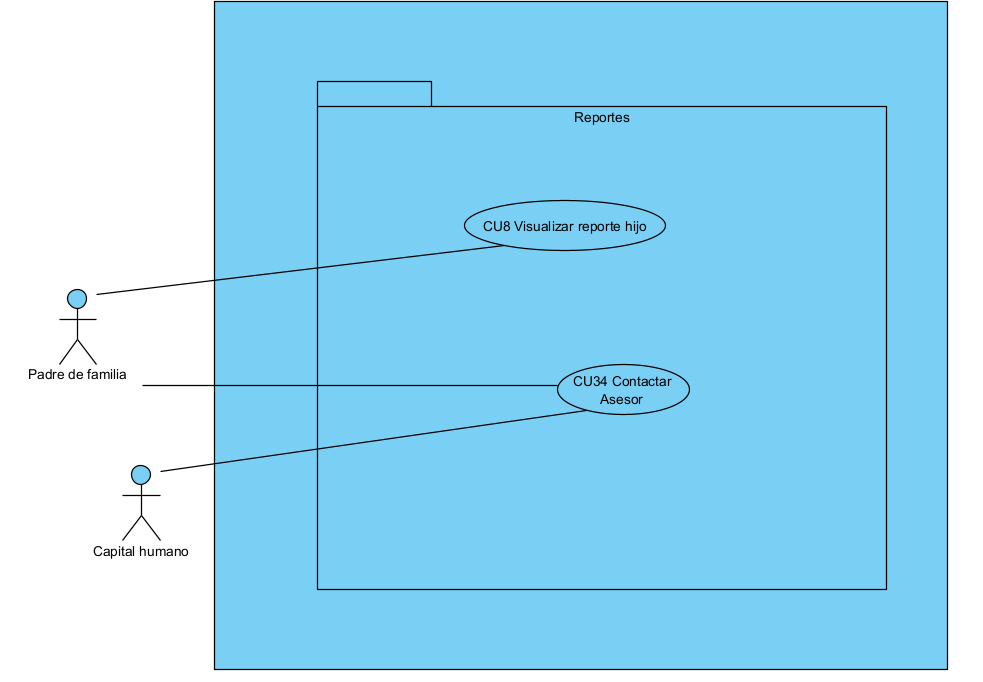
\includegraphics[width=0.7\textwidth]{images/arqui/subSisGestInfantReportes.png}
\caption{Diagrama del Submodulo de reportes.}
\label{fig:subsistGestionInfanReportes}
\end{figure}

\clearpage
%------------------------------------------------------------------
\subsection{Subsistema de Gestión días hábiles}

El subsistema de "Gestión de días hábiles" se encarga de administrar y gestionar los días hábiles, eventos escolares y días inhábiles en la guardería, con el objetivo de asegurar una planificación eficiente y un funcionamiento adecuado del centro.

El subsistema de Gestión de días hábiles consta de dos casos de uso directos, que son los siguientes:

\subsubsection{Registrar evento escolar}
Este caso de uso permite registrar y programar eventos escolares en el calendario de la guardería. Estos eventos pueden incluir actividades especiales, celebraciones, salidas educativas, visitas de invitados, entre otros. Al registrar un evento escolar, se asigna una fecha y se proporciona información relevante como la descripción, los horarios y las personas involucradas. Esto facilita la planificación y organización de las actividades, permitiendo que tanto el personal docente como los padres de familia estén informados y preparados para el evento.

\subsubsection{Registrar día inhábil}
Este caso de uso permite registrar y marcar como día inhábil aquellos días en los que la guardería no estará operativa. Estos días pueden corresponder a feriados, días de descanso programados, mantenimiento o cualquier otra circunstancia que requiera que el centro esté cerrado. Al registrar un día inhábil, se bloquea esa fecha en el calendario de la guardería, evitando la asignación de actividades y la presencia de personal y niños en el centro. Esto permite una gestión adecuada de los recursos y una planificación acorde a los días disponibles de funcionamiento.
\\
El subsistema de Gestión de días hábiles desempeña un papel crucial en la organización y planificación de la guardería "Guardería Burbujas". A través de los casos de uso de registrar eventos escolares y registrar días inhábiles, se establece un calendario que ayuda a mantener la coherencia y la eficiencia en el funcionamiento diario del centro. Esto garantiza que tanto el personal docente como los padres de familia estén al tanto de las actividades programadas y de los días en los que la guardería estará cerrada. En última instancia, este subsistema contribuye a crear un entorno estable y predecible para el desarrollo y cuidado de los infantes en la guardería.


\begin{figure}[htbp]
\centering
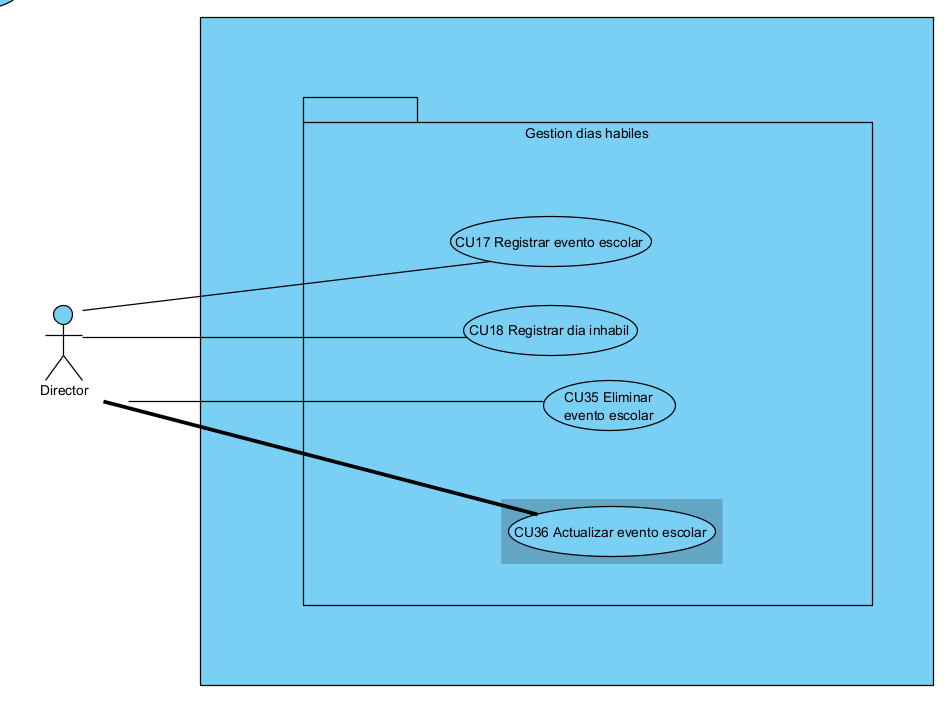
\includegraphics[width=0.7\textwidth]{images/arqui/subSisGestdias.png}
\caption{Diagrama del Subsistema de Gestion dias habiles.}
\label{fig:subsistGestiondias}
\end{figure}
\clearpage
%------------------------------------------------------------------
\subsection{Subsistema de Gestión clases}

El subsistema de "Gestión de clases" es una parte fundamental del sistema de la guardería "Guardería Burbujas". Este subsistema se encarga de la administración y control de las actividades relacionadas con las clases impartidas a los niños en la guardería. El objetivo principal de este subsistema es garantizar un ambiente educativo adecuado y facilitar el proceso de enseñanza-aprendizaje.

El subsistema de Gestión de clases consta de los siguientes submódulos:

\begin{itemize}
\item \textbf{Asistencia}: Este módulo permite realizar el registro y seguimiento de la asistencia de los niños a las clases. El profesor puede marcar la asistencia de cada estudiante y mantener un registro actualizado de su asistencia diaria. Esto facilita el control de la asistencia y proporciona información valiosa para evaluar la participación y el progreso de los niños en las actividades escolares.

\item \textbf{Reporte}: El módulo de Reporte permite generar informes y reportes sobre el desempeño y el progreso de los niños en las clases. El profesor puede ingresar datos relevantes, como calificaciones, observaciones y comentarios sobre el rendimiento de cada estudiante. Estos informes son útiles para evaluar el desarrollo de los niños, comunicarse con los padres y tomar decisiones educativas informadas.

\item \textbf{Avisos}: El módulo de Avisos es una herramienta de comunicación entre el profesor y los padres. Permite enviar notificaciones, recordatorios y mensajes importantes relacionados con las clases y el progreso de los niños. Los profesores pueden compartir información relevante, como fechas de eventos, tareas o cualquier otra comunicación necesaria para mantener una buena comunicación con los padres y garantizar su participación activa en la educación de sus hijos.

\end{itemize}

El actor principal que interactúa con el subsistema de Gestión de clases es el profesor. El profesor utiliza los diferentes módulos para tomar el control de las clases, registrar la asistencia de los niños, evaluar su desempeño y comunicarse de manera efectiva con los padres. A través de este subsistema, se busca promover un entorno educativo dinámico y propicio para el crecimiento y desarrollo de los niños en la guardería "Guardería Burbujas".


\begin{figure}[htbp]
\centering
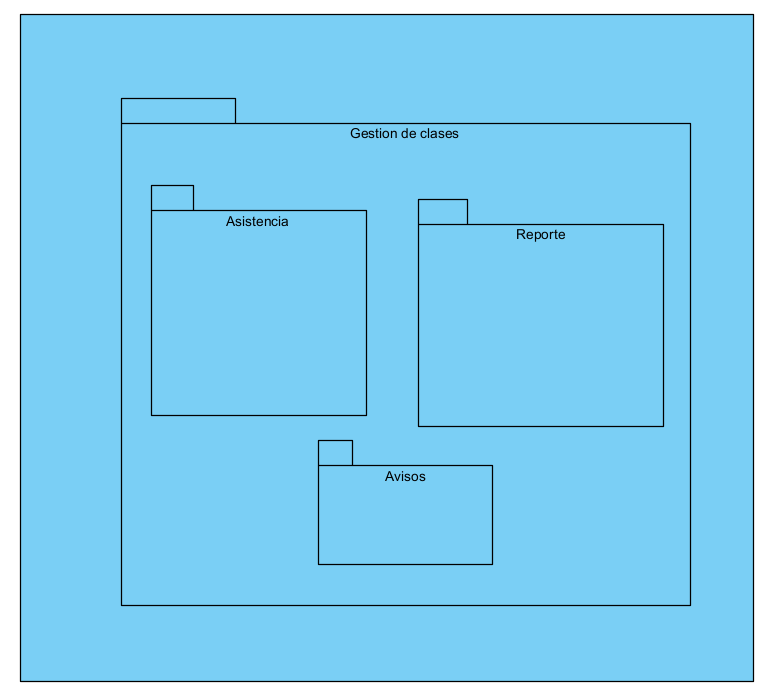
\includegraphics[width=0.7\textwidth]{images/arqui/subSisGestClases.png}
\caption{Diagrama del Subsistema de Gestion de Clases.}
\label{fig:subsistGestionClases}
\end{figure}

\subsubsection{Submódulo de Asistencia}

Este submódulo se encarga de realizar el registro y seguimiento de la asistencia de los niños a las clases, así como de registrar su salida al finalizar la jornada escolar. Su objetivo principal es mantener un control preciso y actualizado de la asistencia de los niños, lo que facilita la organización de las clases y proporciona información valiosa sobre su participación en las actividades escolares.

El submódulo de Asistencia ofrece las siguientes funcionalidades:

\begin{itemize}
\item \textbf{Tomar asistencia}: Esta funcionalidad permite al profesor tomar la asistencia de los niños al comienzo de cada clase. El profesor puede registrar la presencia o ausencia de cada estudiante, lo cual se refleja en el sistema. Esta información se utiliza para mantener un registro actualizado de la asistencia y generar informes precisos sobre la participación de los niños en las clases.

\item \textbf{Registrar salida}: Al finalizar la jornada escolar, el profesor puede registrar la salida de los niños en el submódulo de Asistencia. Esto asegura que se tenga un registro completo de las horas de asistencia de cada niño y brinda a los padres la tranquilidad de saber que sus hijos han sido debidamente registrados al ingresar y salir de la guardería.
\end{itemize}




\begin{figure}[htbp]
\centering
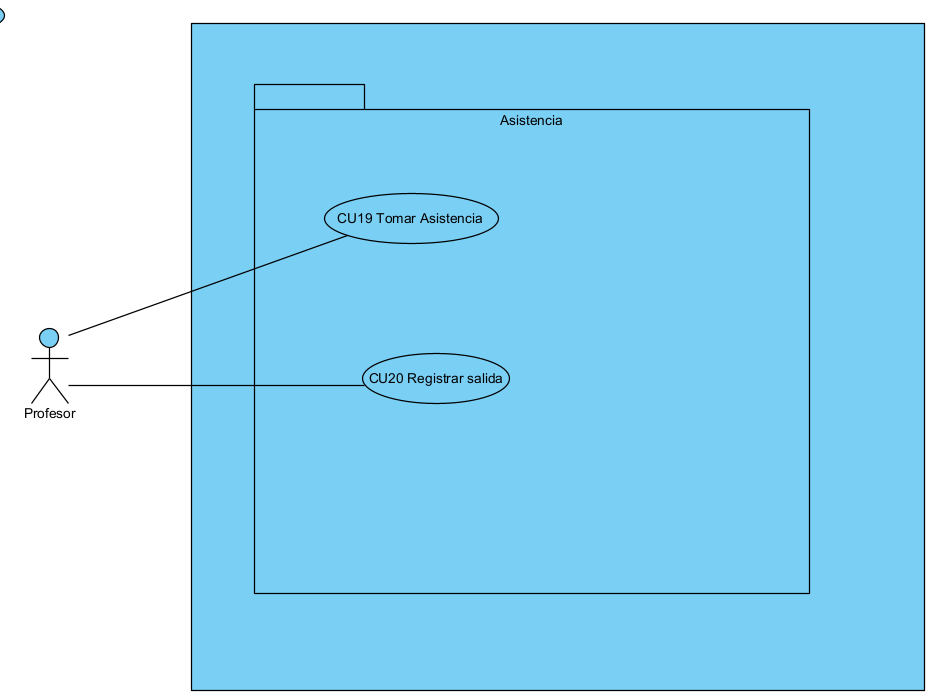
\includegraphics[width=0.7\textwidth]{images/arqui/subSisGestClasesAsis.png}
\caption{Diagrama del Submodulo de Asistencia.}
\label{fig:subsistGestionClasesAsis}
\end{figure}


\subsubsection{Submódulo de Avisos}

tiene como objetivo facilitar la comunicación entre el profesor y los padres de familia, brindando un canal eficiente para enviar y recibir avisos relevantes sobre actividades, eventos o cualquier otra información importante relacionada con la educación y el bienestar de los niños.

El submódulo de Avisos ofrece las siguientes funcionalidades:

\begin{itemize}
\item \textbf{Solicitar material}: Mediante esta funcionalidad, el profesor puede enviar avisos a los padres de familia solicitando materiales específicos para actividades escolares. Por ejemplo, si se va a realizar una manualidad, el profesor puede solicitar a los padres que envíen ciertos materiales como papel, pegamento, tijeras, entre otros. Esta funcionalidad agiliza el proceso de comunicación y permite al profesor asegurarse de contar con los recursos necesarios para llevar a cabo las actividades planificadas.

\item \textbf{Contactar padre de familia}: Esta funcionalidad permite al profesor establecer comunicación directa con los padres de familia para tratar asuntos específicos relacionados con los niños. Puede ser utilizada para compartir información personalizada, responder preguntas o resolver cualquier inquietud que pueda surgir. La capacidad de contactar directamente a los padres de familia a través del submódulo de Avisos fomenta una comunicación fluida y eficiente entre ambas partes, promoviendo una colaboración activa en la educación y cuidado de los niños.

\end{itemize}

\begin{figure}[htbp]
\centering
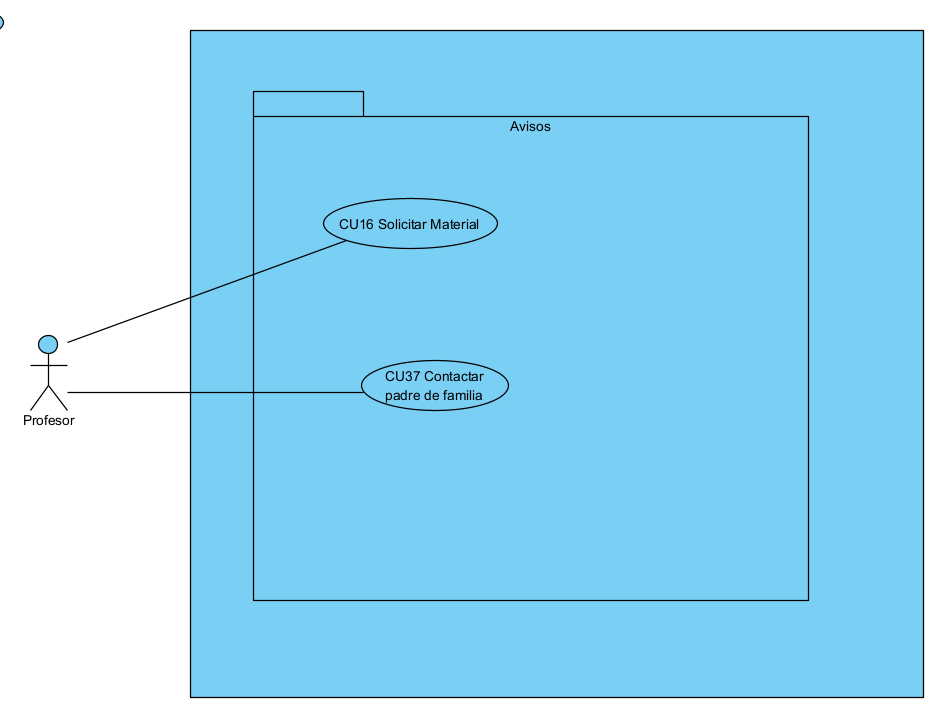
\includegraphics[width=0.7\textwidth]{images/arqui/subSisGestClasesAvis.png}
\caption{Diagrama del Submodulo de Avisos.}
\label{fig:subsistGestionClasesAvis}
\end{figure}

\subsubsection{Submódulo de Reportes}
El submódulo de Reportes es una parte esencial del subsistema de Gestión de clases en la guardería "Guardería Burbujas" se encarga de recopilar y registrar información relevante sobre diferentes aspectos relacionados con el cuidado y el desarrollo de los niños durante su estancia en la guardería.

El submódulo de Reportes ofrece las siguientes funcionalidades:

\begin{itemize}
\item \textbf{Registrar evacuaciones}: Esta funcionalidad permite al profesor registrar y documentar las evacuaciones realizadas por cada niño. Se registra información como la fecha, hora y características de la evacuación, lo cual es importante para llevar un control adecuado de la salud y bienestar de los infantes.

\item \textbf{Registrar ingesta}: Mediante esta funcionalidad, el profesor puede registrar la información sobre la ingesta de alimentos y bebidas de cada niño durante su estancia en la guardería. Se registra el tipo de alimento, la cantidad y cualquier otra observación relevante relacionada con la alimentación de los niños.

\item \textbf{Registrar cambio de ropa}: Esta funcionalidad permite al profesor registrar cualquier cambio de ropa que deba realizarse a un niño durante el día. Se registra la fecha, hora y motivo del cambio de ropa, lo cual es útil para mantener un seguimiento adecuado de las necesidades individuales de los niños.

\item \textbf{Registrar información adicional}: Esta funcionalidad permite al profesor registrar cualquier información adicional relevante sobre los niños. Puede incluir observaciones específicas, comportamientos destacados, eventos especiales o cualquier otra información que sea importante para comprender y atender las necesidades de los niños de manera individualizada.

\item \textbf{Generar reporte}: Una vez registrada la información en los submódulos anteriores, el profesor puede utilizar esta funcionalidad para generar un reporte consolidado. El reporte contiene un resumen de la información registrada en cuanto a evacuaciones, ingesta, cambios de ropa, información adicional, tareas y actividades realizadas por los niños. Estos reportes pueden ser utilizados para compartir información con los padres de familia, evaluar el progreso de los niños y realizar un seguimiento adecuado de su desarrollo.

\item \textbf{Registrar tareas y actividades}: Esta funcionalidad permite al profesor registrar las tareas y actividades que se realizan con los niños durante su estancia en la guardería. Se registra información como el tipo de tarea o actividad, la fecha, la duración y cualquier observación relevante. Esto facilita la planificación y organización de las actividades educativas y recreativas para el beneficio de los niños.

\end{itemize}

El submódulo de Reportes del subsistema de Gestión de clases juega un papel fundamental en la recopilación, registro y generación de información relevante sobre el cuidado y desarrollo de los niños en la guardería. Al utilizar este submódulo, se garantiza una documentación adecuada de las evacuaciones, la ingesta de alimentos, los cambios de ropa, la información adicional, las tareas y las actividades realizadas por los niños. Esto contribuye a la evaluación integral de su progreso, el seguimiento de sus necesidades individuales y la comunicación


\begin{figure}[htbp]
\centering
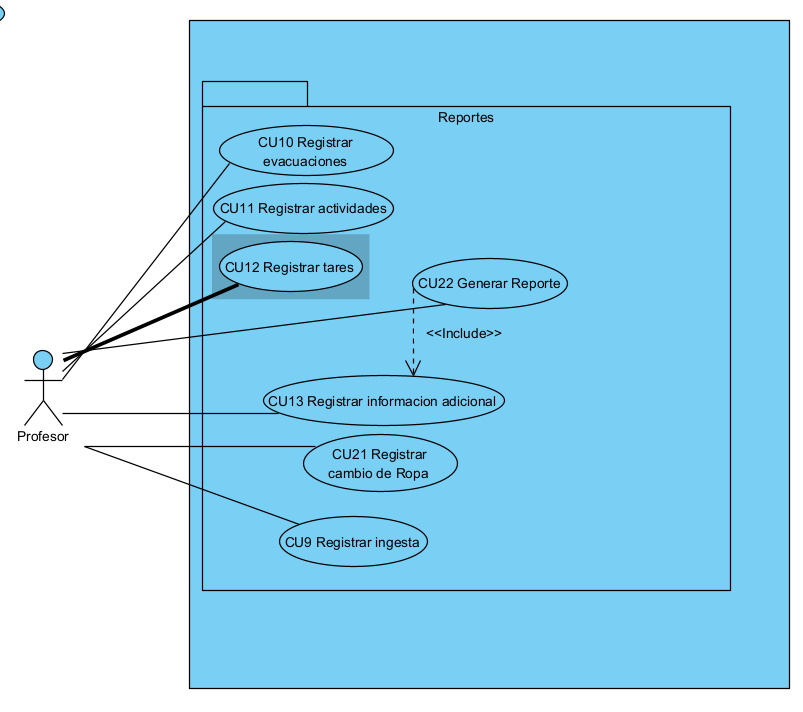
\includegraphics[width=0.7\textwidth]{images/arqui/subSisGestClasesRepor.png}
\caption{Diagrama del Submodulo de Reportes.}
\label{fig:subsistGestionClasesRepor}
\end{figure}


\clearpage
%------------------------------------------------------------------
\subsection{Subsistema Salud}

El subsistema de Salud es una parte fundamental del sistema de la guardería "Guardería Burbujas". Este subsistema se encarga de garantizar el bienestar y la salud de los niños que asisten a la guardería. En este subsistema, se involucran dos actores principales: el Médico y el Nutriólogo.\\

El Médico es responsable de llevar a cabo acciones relacionadas con la salud de los niños. Esto incluye generar consultas médicas, evaluar el estado de salud de los infantes, realizar diagnósticos, prescribir medicamentos y llevar un registro de las incidencias médicas de cada niño. El Médico juega un papel crucial en el cuidado y la atención médica de los niños, asegurándose de que estén sanos y respondiendo de manera adecuada a cualquier problema de salud que puedan presentar.

Por otro lado, el Nutriólogo desempeña un papel importante en el aspecto nutricional de los niños. Su tarea principal es crear los menús balanceados y adecuados para cada niño, teniendo en cuenta sus necesidades dietéticas individuales, alergias, preferencias y restricciones alimentarias. El Nutriólogo se asegura de proporcionar una alimentación saludable y equilibrada, promoviendo hábitos alimentarios saludables y fomentando el bienestar nutricional de los niños.

\begin{figure}[htbp]
\centering
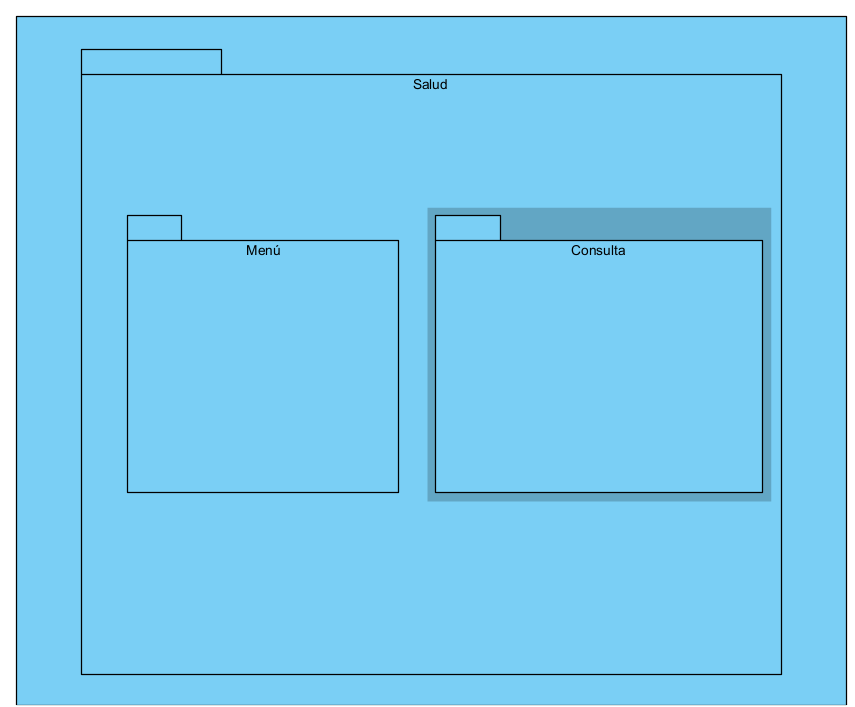
\includegraphics[width=0.7\textwidth]{images/arqui/subSalud.png}
\caption{Subsistema Salud.}
\label{fig:subsistsalud}
\end{figure}

\subsubsection{Submódulo de Menu}
La subsección "Menú" dentro del subsistema de Salud se encarga de gestionar las acciones relacionadas con la creación y registro de menús para los niños en la guardería "Guardería Burbujas". Este módulo es fundamental para garantizar una alimentación adecuada y equilibrada para los infantes, asegurando que se cumplan sus necesidades nutricionales.

El módulo del Menú permite realizar las siguientes acciones:

\begin{itemize}
    \item[*] Registro de menú: En esta funcionalidad, el nutriólogo encargado puede registrar los menús diarios o semanales para los diferentes grupos de niños. El nutriólogo puede seleccionar los alimentos adecuados y planificar las comidas de acuerdo con las necesidades nutricionales y restricciones dietéticas de cada niño.
    \item[*] Creación de menú especial: En algunos casos, es posible que se requiera crear menús especiales para niños con necesidades dietéticas específicas, como alergias o intolerancias alimentarias. El nutriólogo puede diseñar menús especiales adaptados a las necesidades individuales de cada niño, garantizando su seguridad y bienestar.
    \item[*] Visualización de menú: El nutriologo pueden acceder a la visualización de los menús registrados. Esta funcionalidad les permite planear de antemano las comidas que se servirán a los niños en la guardería, lo que les brinda tranquilidad y les permite tomar decisiones informadas sobre la alimentación de los infantes

\end{itemize}

\begin{figure}[htbp]
\centering
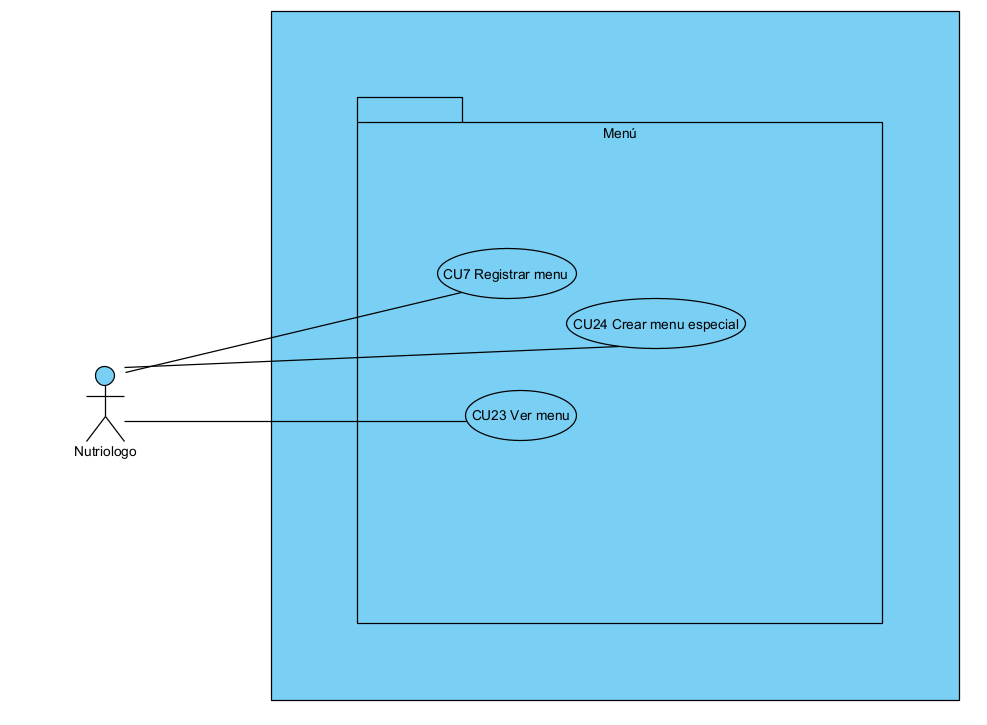
\includegraphics[width=0.7\textwidth]{images/arqui/subSaludMenu.png}
\caption{Modulo del Menu del subsistema Salud.}
\label{fig:subsistsaludmenu}
\end{figure}



\subsubsection{Submódulo de Consulta}
La subsección "Consulta" dentro del subsistema de Salud se encarga de gestionar las acciones relacionadas con la atención médica y el registro de incidencias médicas en la guardería "Guardería Burbujas". Este módulo es fundamental para asegurar el cuidado y bienestar de los niños, proporcionando un seguimiento adecuado de su estado de salud.

El módulo de Consulta permite realizar las siguientes acciones:

\begin{itemize}
\item[*] Registro de incidencia médica: En esta funcionalidad, el médico de la guardería puede registrar y documentar cualquier incidencia o situación médica que ocurra con un niño. Esto incluye enfermedades, lesiones, alergias u otras condiciones de salud relevantes. El médico puede ingresar detalles sobre el diagnóstico, tratamiento, medicamentos recetados y cualquier recomendación adicional para el cuidado del niño.


\end{itemize}

\begin{figure}[htbp]
\centering
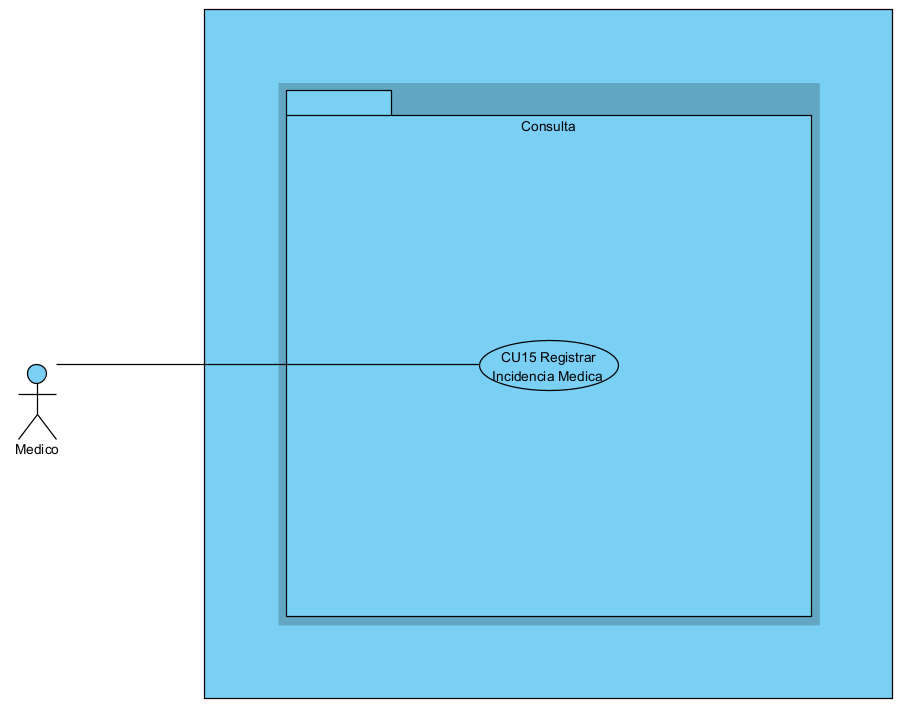
\includegraphics[width=0.7\textwidth]{images/arqui/subSaludConsulta.png}
\caption{Modulo de Consulta del subsistema Salud.}
\label{fig:subsistsaludcons}
\end{figure}
\clearpage


%==========================================================================
%-----------------------------------------------------------------------
\section{Diseño de clases}

El diseño de clases es una etapa esencial en el desarrollo de software basado en programación orientada a objetos (POO). En esta sección, nos centraremos en el diseño de clases relacionadas con diferentes entidades que forman parte de un sistema. Estas entidades incluyen a capital humano, los recursos humanos, los reportes, el menú de comidas, los padres de familia, los infantes, el director, el médico, el nutriólogo y el profesor.\\

En esta sección, abordaremos el diseño de clases para cada una de estas entidades, definiendo sus atributos, métodos y relaciones con otras clases. Un diseño de clases bien estructurado y coherente es fundamental para construir un sistema robusto y escalable, que cumpla con los requisitos y funcionalidades deseadas.


\begin{figure}[htbp]
\centering
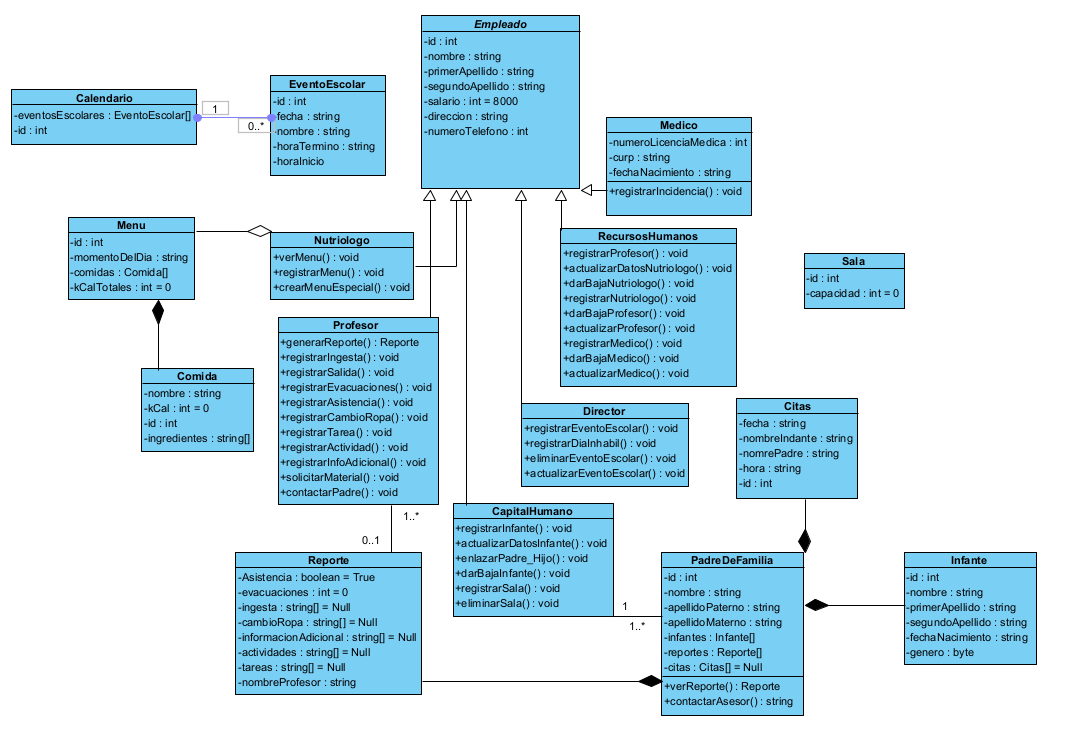
\includegraphics[width=0.9\textwidth]{images/arqui/entidades.png}
\caption{Diagrama de entidades del sistema.}
\label{fig:entidades}
\end{figure}
\clearpage

\subsection{Empleado}

En esta subsección, se aborda el diseño de la clase abstracta que representa a un empleado dentro del sistema. Un empleado es una entidad fundamental en cualquier organización y puede tener diferentes roles y responsabilidades. A continuación, se definen los atributos principales de la clase abstracta \texttt{Empleado}.

La clase abstracta \texttt{Empleado} contiene los siguientes atributos:

\begin{itemize}
\item \texttt{nombre}: Representa el nombre del empleado, que puede incluir su primer nombre o nombres.

\item \texttt{apellidoPaterno}: Indica el apellido paterno del empleado, que forma parte de su nombre completo.

\item \texttt{apellidoMaterno}: Representa el apellido materno del empleado, que también forma parte de su nombre completo.

\item \texttt{salario}: Indica la remuneración económica o sueldo que recibe el empleado por su trabajo.

\item \texttt{direccion}: Representa la ubicación física o geográfica donde el empleado desempeña sus funciones dentro de la organización.


\item \texttt{numeroTelefono}: Es el número de contacto telefónico del empleado, utilizado para comunicaciones y coordinación.

\item \texttt{id}: Es un identificador único asignado al empleado dentro del sistema, que se utiliza para realizar operaciones y realizar seguimiento de su información.

\end{itemize}

La clase abstracta \texttt{Empleado} se utiliza como base para definir clases más específicas que representan diferentes tipos de empleados en el sistema, como \texttt{Director}, \texttt{Medico}, \texttt{Nutriologo} y otros. Al ser una clase abstracta, no se puede instanciar directamente, pero proporciona una estructura común y atributos compartidos para las clases derivadas.

\begin{figure}[htbp]
\centering
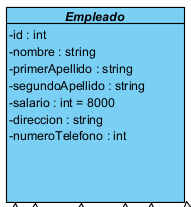
\includegraphics[width=0.4\textwidth]{images/arqui/empleado.png}
\caption{Diagrama de la clase abstracta empleado.}
\label{fig:entidadempleado}
\end{figure}
\clearpage
%------------------------------------------------------------------
\subsection{Nutriólogo}

La entidad \texttt{Nutriologo}, que es una subclase de la clase abstracta \texttt{Empleado}. El nutriólogo es un tipo específico de empleado que se especializa en la planificación y supervisión de la alimentación y nutrición de los infantes en la guardería "Guardería Burbujas".

La clase \texttt{Nutriologo} hereda los atributos de la clase \texttt{Empleado}, que incluyen:

\begin{itemize}
\item \textbf{nombre}: el nombre del nutriólogo.
\item \textbf{apellido paterno}: el apellido paterno del nutriólogo.
\item \textbf{apellido materno}: el apellido materno del nutriólogo.

\item \textbf{salario}: el salario del nutriólogo.
\item \textbf{ubicación}: la ubicación del nutriólogo en la guardería.

\item \textbf{número de teléfono}: el número de teléfono del nutriólogo.
\item \textbf{id}: el identificador único del nutriólogo en el sistema.
\end{itemize}

La clase \texttt{Nutriologo} también tiene los siguientes métodos:

\begin{itemize}
\item \textbf{verMenú()}: este método permite al nutriólogo ver el menú registrado para los infantes en la guardería. Proporciona al nutriólogo una visión general de las comidas planificadas y les permite realizar ajustes si es necesario.
\item \textbf{crearMenúEspecial()}: este método permite al nutriólogo crear un menú especial para un infante con necesidades dietéticas específicas, como alergias o intolerancias alimentarias. El nutriólogo puede diseñar un menú adaptado a las necesidades individuales del infante, asegurando una alimentación segura y saludable.
\item \textbf{registrarMenú()}: este método permite al nutriólogo registrar el menú diario o semanal para los infantes en la guardería. El nutriólogo puede seleccionar los alimentos adecuados y planificar las comidas de acuerdo con las necesidades nutricionales y restricciones dietéticas de cada infante.
\end{itemize}

La clase \texttt{Nutriologo} desempeña un papel fundamental en el subsistema de gestión de personal de la guardería "Guardería Burbujas". Con su experiencia y conocimientos en nutrición, contribuye a garantizar una alimentación adecuada y equilibrada para los infantes, promoviendo su bienestar y desarrollo saludable.


\begin{figure}[htbp]
\centering
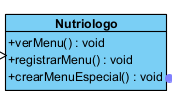
\includegraphics[width=0.4\textwidth]{images/arqui/nutriologo.png}
\caption{Diagrama de la clase anutriologo.}
\label{fig:entidadNutriologo}
\end{figure}

\clearpage
%------------------------------------------------------------------
\subsection{Medico}

La entidad \texttt{Médico}, que es una subclase de la clase abstracta \texttt{Empleado}. El médico es un tipo específico de empleado que brinda atención médica y cuidado de la salud a los infantes en la guardería "Guardería Burbujas".

La clase \texttt{Médico} hereda los atributos de la clase \texttt{Empleado}, que incluyen:

\begin{itemize}
\item \textbf{nombre}: el nombre del médico.
\item \textbf{apellido paterno}: el apellido paterno del médico.
\item \textbf{apellido materno}: el apellido materno del médico.

\item \textbf{salario}: el salario del médico.
\item \textbf{direccion}: la ubicación del médico en la guardería.

\item \textbf{número de teléfono}: el número de teléfono del médico.
\item \textbf{id }: el identificador único del médico en el sistema.
\end{itemize}

Además, la clase \texttt{Médico} tiene el atributo adicional:

\begin{itemize}
\item \textbf{numeroLicenciaMedica}: el número de licencia médica del médico, que identifica su autorización legal para ejercer la medicina.
\end{itemize}

La clase \texttt{Médico} también tiene el siguiente método:

\begin{itemize}
\item \textbf{registrarIncidencia()}: este método permite al médico registrar incidencias o eventos médicos relacionados con los infantes en la guardería. Puede incluir registros de enfermedades, lesiones o cualquier otra situación médica relevante. El médico puede proporcionar detalles y seguimiento adecuado para garantizar la salud y el bienestar de los infantes.
\end{itemize}

La clase \texttt{Médico} desempeña un papel crucial en el cuidado de la salud de los infantes en la guardería "Guardería Burbujas". Su experiencia médica y conocimientos permiten una atención adecuada en caso de enfermedad, lesiones o situaciones médicas imprevistas. Trabaja en estrecha colaboración con el personal y los padres de familia para garantizar un entorno seguro y saludable para los infantes.+

\begin{figure}[htbp]
\centering
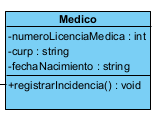
\includegraphics[width=0.4\textwidth]{images/arqui/medico.png}
\caption{Diagrama de la clase del Medico.}
\label{fig:entidadMedico}
\end{figure}

\clearpage
%------------------------------------------------------------------
\subsection{Profesor}
La entidad \texttt{Profesor}, que es una subclase de la clase abstracta \texttt{Empleado}. El profesor es un tipo específico de empleado que se encarga del cuidado y la educación de los infantes en la guardería "Guardería Burbujas".

La clase \texttt{Profesor} hereda los atributos de la clase \texttt{Empleado}, que incluyen:

\begin{itemize}
\item \textbf{nombre}: el nombre del profesor.
\item \textbf{apellido paterno}: el apellido paterno del profesor.
\item \textbf{apellido materno}: el apellido materno del profesor.

\item \textbf{salario}: el salario del profesor.
\item \textbf{direccion}: la ubicación del profesor en la guardería.

\item \textbf{número de teléfono}: el número de teléfono del profesor.
\item \textbf{id}: el identificador único del profesor en el sistema.
\end{itemize}

Además, la clase \texttt{Profesor} tiene los siguientes atributos adicionales:

\begin{itemize}
\item \textbf{registrarReporte}: este atributo representa la capacidad del profesor para registrar reportes sobre el progreso y el comportamiento de los infantes.
\item \textbf{registrarIngesta}: este atributo indica la capacidad del profesor para registrar la ingesta de alimentos de los infantes durante las comidas.
\item \textbf{registrarSalida}: este atributo permite al profesor registrar la hora de salida de los infantes al final del día.
\item \textbf{registrarEvacuaciones}: este atributo representa la capacidad del profesor para registrar las evacuaciones o visitas al baño de los infantes.
\item \textbf{registrarAsistencia}: este atributo indica la capacidad del profesor para registrar la asistencia de los infantes en la guardería.
\item \textbf{registrarCambioRopa}: este atributo permite al profesor registrar los cambios de ropa de los infantes, por ejemplo, después de actividades o en caso de accidentes.
\item \textbf{registrarTarea}: este atributo representa la capacidad del profesor para registrar las tareas asignadas a los infantes, como actividades de aprendizaje o tareas creativas.
\item \textbf{registrarActividad}: este atributo indica la capacidad del profesor para registrar las actividades realizadas por los infantes, como juegos, ejercicios o proyectos.
\item \textbf{registrarInfoAdicional}: este atributo permite al profesor registrar información adicional relevante sobre los infantes, como notas de comportamiento, preferencias o necesidades especiales.
\item \textbf{solicitarMaterial}: este atributo representa la capacidad del profesor para solicitar material o recursos necesarios para las actividades y el cuidado de los infantes.
\item \textbf{contactarPadre}: este atributo indica la capacidad del profesor para contactar a los padres de familia en caso de situaciones importantes, actualizaciones o consultas relacionadas con los infantes.
\end{itemize}

La clase \texttt{Profesor} desempeña un papel vital en el cuidado y la educación de los infantes en la guardería "Guardería Burbujas". Su responsabilidad incluye la supervisión, el apoyo y la instrucción de los infantes durante su estancia en la guardería. El profesor trabaja en estrecha colaboración con el personal y los padres de familia para garantizar el bienestar, el desarrollo y el aprendizaje de los infantes en un entorno seguro y estimulante.


\begin{figure}[htbp]
\centering
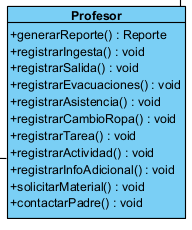
\includegraphics[width=0.4\textwidth]{images/arqui/profesor.png}
\caption{Diagrama de la clase del profesor.}
\label{fig:entidadProfesor}
\end{figure}

\clearpage
%------------------------------------------------------------------
\subsection{Capital Humano}

\texttt{CapitalHumano}, que es una subclase de la clase abstracta \texttt{Empleado}. La clase \texttt{CapitalHumano} se encarga de la gestión y administración de los recursos humanos relacionados con el cuidado de los infantes en la guardería "Guardería Burbujas".

La clase \texttt{CapitalHumano} hereda los atributos y métodos de la clase \texttt{Empleado}, y también tiene los siguientes métodos adicionales:

\begin{itemize}
\item \texttt{registrarInfante}: Este método permite registrar a un nuevo infante en el sistema. Se recopilan los datos necesarios del infante, como nombre, apellido, CURP, ubicación, edad, número de teléfono y ID en el sistema. Estos datos se utilizan para crear una nueva instancia de la clase \texttt{Infante} y agregarla al registro de infantes.

\item \texttt{actualizarDatosInfante}: Este método permite actualizar los datos de un infante registrado en el sistema. Se identifica al infante por su ID en el sistema y se actualizan los atributos correspondientes, como nombre, apellido, CURP, ubicación, edad y número de teléfono.

\item \texttt{enlazarPadre\_Hijo}: Este método permite establecer una relación entre un padre de familia y su hijo en el sistema. Se recopilan los datos del padre de familia y del infante, y se realiza el enlace correspondiente en el registro de padres e infantes.

\item \texttt{darBajaInfante}: Este método permite dar de baja a un infante del sistema. Se realiza mediante la identificación del infante por su ID en el sistema y eliminando su instancia correspondiente del registro de infantes.

\item \texttt{registrarSala}: Este método permite registrar una nueva sala en el sistema. Se recopilan los datos necesarios de la sala, como nombre, capacidad y ubicación, y se crea una nueva instancia de la clase \texttt{Sala} para agregarla al registro de salas.

\item \texttt{eliminarSala}: Este método permite eliminar una sala del sistema. Se realiza mediante la identificación de la sala por su ID en el sistema y eliminando su instancia correspondiente del registro de salas.
\end{itemize}

\begin{figure}[htbp]
\centering
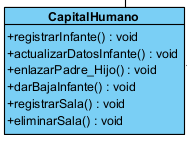
\includegraphics[width=0.4\textwidth]{images/arqui/capitalhumano.png}
\caption{Diagrama de la clase del Capital humano.}
\label{fig:entidadCaH}
\end{figure}

\clearpage
%------------------------------------------------------------------
\subsection{Director}

\texttt{Director}, que es una subclase de la clase abstracta \texttt{Empleado}. La clase \texttt{Director} representa al director de la guardería "Guardería Burbujas" y se encarga de la gestión y supervisión general de la institución.

La clase \texttt{Director} hereda los atributos y métodos de la clase \texttt{Empleado}, y también tiene los siguientes métodos adicionales:

\begin{itemize}
\item \texttt{registrarEventoEscolar}: Este método permite registrar un evento escolar en el sistema. Se recopilan los datos del evento, como el nombre, la fecha, la descripción y cualquier otra información relevante. El evento se agrega al registro de eventos escolares y se asocia con los infantes y el personal correspondiente.

\item \texttt{registrarDiaInhabil}: Este método permite registrar un día inhabil en el sistema. Se especifica la fecha y se agrega al registro de días inhabiles. Esto puede ser útil para planificar días en los que la guardería estará cerrada o no se ofrecerán servicios regulares.

\item \texttt{eliminarEventoEscolar}: Este método permite eliminar un evento escolar del sistema. Se realiza mediante la identificación del evento por su ID en el sistema y eliminando su instancia correspondiente del registro de eventos escolares.

\item \texttt{actualizarEventoEscolar}: Este método permite actualizar los datos de un evento escolar registrado en el sistema. Se identifica el evento por su ID en el sistema y se actualizan los atributos correspondientes, como el nombre, la fecha, la descripción y cualquier otra información relevante.

\end{itemize}



\begin{figure}[htbp]
\centering
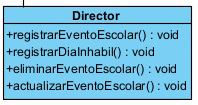
\includegraphics[width=0.4\textwidth]{images/arqui/director.png}
\caption{Diagrama de la clase director.}
\label{fig:entidadDirector}
\end{figure}

\clearpage
%------------------------------------------------------------------
\subsection{Recursos humanos}

\texttt{RecursosHumanos}, que es una subclase de la clase abstracta \texttt{Empleado}. La clase \texttt{RecursosHumanos} se encarga de la gestión y administración del personal en la guardería "Guardería Burbujas".

La clase \texttt{RecursosHumanos} hereda los atributos y métodos de la clase \texttt{Empleado}, y también tiene los siguientes métodos adicionales:

\begin{itemize}
\item \texttt{registrarProfesor}: Este método permite registrar a un nuevo profesor en el sistema. Se recopilan los datos necesarios del profesor, como nombre, apellido, CURP, salario, ubicación, edad, número de teléfono y ID en el sistema. Estos datos se utilizan para crear una nueva instancia de la clase \texttt{Profesor} y agregarla al registro de profesores.

\item \texttt{darBajaProfesor}: Este método permite dar de baja a un profesor del sistema. Se realiza mediante la identificación del profesor por su ID en el sistema y eliminando su instancia correspondiente del registro de profesores.

\item \texttt{actualizarDatosProfesor}: Este método permite actualizar los datos de un profesor registrado en el sistema. Se identifica al profesor por su ID en el sistema y se actualizan los atributos correspondientes, como nombre, apellido, CURP, salario, ubicación, edad y número de teléfono.

\item \texttt{actualizarDatosNutriologo}: Este método permite actualizar los datos de un nutriólogo registrado en el sistema. Se identifica al nutriólogo por su ID en el sistema y se actualizan los atributos correspondientes, como nombre, apellido, CURP, salario, ubicación, edad y número de teléfono.

\item \texttt{registrarNutriologo}: Este método permite registrar a un nuevo nutriólogo en el sistema. Se recopilan los datos necesarios del nutriólogo, como nombre, apellido, CURP, salario, ubicación, edad, número de teléfono y ID en el sistema. Estos datos se utilizan para crear una nueva instancia de la clase \texttt{Nutriologo} y agregarla al registro de nutriólogos.

\item \texttt{darBajaNutriologo}: Este método permite dar de baja a un nutriólogo del sistema. Se realiza mediante la identificación del nutriólogo por su ID en el sistema y eliminando su instancia correspondiente del registro de nutriólogos.

\item \texttt{actualizarDatosMedico}: Este método permite actualizar los datos de un médico registrado en el sistema. Se identifica al médico por su ID en el sistema y se actualizan los atributos correspondientes, como nombre, apellido, CURP, salario, ubicación, edad y número de teléfono.

\item \texttt{registrarMedico}: Este método permite registrar a un nuevo médico en el sistema. Se recopilan los datos necesarios del médico, como nombre, apellido, CURP, salario, ubicación, edad, número de teléfono y ID en el sistema. Estos datos se utilizan para crear una nueva instancia de la clase \texttt{Medico} y agregarla al registro de médicos.

\item \texttt{darBajaMedico}: Este método permite dar de baja a un médico del sistema. Se realiza mediante la identificación del médico por su ID en el sistema y eliminando su instancia correspondiente del registro de médicos.
\end{itemize}

\begin{figure}[htbp]
\centering
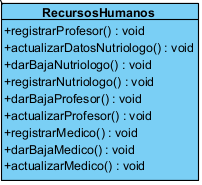
\includegraphics[width=0.4\textwidth]{images/arqui/recursoshumanos.png}
\caption{Diagrama de la clase recursos humanos.}
\label{fig:entidadRH}
\end{figure}

\clearpage
%------------------------------------------------------------------
\subsection{Padre de familia}
\texttt{Padre de familia}, que representa a los padres o tutores de los infantes inscritos en la guardería "Guardería Burbujas". Los padres de familia son parte integral del sistema y desempeñan un papel importante en la comunicación y el seguimiento del progreso de sus hijos.

La entidad \texttt{Padre de familia} tiene los siguientes atributos:

\begin{itemize}
\item \texttt{id}: Identificador único del padre de familia.
\item \texttt{nombre, apellidos}: El nombre y apellidos del padre de familia.
\item \texttt{infantes}: Una lista que contiene los infantes asociados a este padre de familia. Cada infante está representado por un objeto de la clase \texttt{Infante}.
\end{itemize}

Además, la entidad \texttt{Padre de familia} tiene los siguientes métodos:

\begin{itemize}
\item \texttt{verReporte}: Este método permite al padre de familia ver el reporte del progreso y desarrollo de sus infantes. El reporte puede incluir información sobre la asistencia, la alimentación, las actividades realizadas y cualquier otra observación relevante sobre el infante.

\item \texttt{contactarAsesor}: Este método permite al padre de familia contactar al asesor o profesor encargado del cuidado y educación del infante. El padre de familia puede utilizar este método para realizar consultas, programar reuniones o comunicar cualquier inquietud o necesidad relacionada con su hijo.

\end{itemize}

Estos métodos facilitan la interacción y comunicación entre los padres de familia y el personal de la guardería, promoviendo una colaboración efectiva en el cuidado y desarrollo de los infantes. Los atributos de la entidad \texttt{Padre de familia} permiten mantener un registro y una asociación adecuada entre los padres y sus hijos inscritos en la guardería.


\begin{figure}[htbp]
\centering
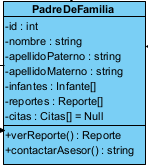
\includegraphics[width=0.4\textwidth]{images/arqui/padreFamilia.png}
\caption{Diagrama de la clase padre de familia.}
\label{fig:entidadpadre}
\end{figure}
\clearpage
%------------------------------------------------------------------
\subsection{Infante}
\texttt{Infante}, que representa a los niños inscritos en la guardería "Guardería Burbujas". Los infantes son el enfoque principal del sistema, ya que se centra en su cuidado, educación y bienestar.

La entidad \texttt{Infante} tiene los siguientes atributos:

\begin{itemize}
\item \texttt{id}: Identificador único del infante.
\item \texttt{nombre, apellidos}: El nombre y apellidos del infante.
\item \texttt{fechaNacimiento}: La fecha de nacimiento del infante.
\item \texttt{género}: El género del infante, que puede ser masculino, femenino o cualquier otra categoría aplicable.
\end{itemize}

Además de estos atributos, la entidad \texttt{Infante} puede tener otros atributos adicionales según las necesidades específicas del sistema, como información médica relevante, alergias, requerimientos especiales, entre otros.

No se especifican métodos específicos para la entidad \texttt{Infante} en esta descripción, ya que los métodos y funcionalidades relacionadas con el cuidado y la gestión de los infantes pueden ser implementados en las clases que heredan de esta entidad, como el \texttt{Profesor} o el \texttt{Padre de familia}.

\begin{figure}[htbp]
\centering
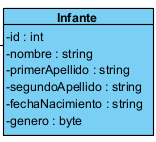
\includegraphics[width=0.4\textwidth]{images/arqui/infante.png}
\caption{Diagrama de la clase infante.}
\label{fig:entidadinfan}
\end{figure}


\begin{figure}[htbp]
\centering
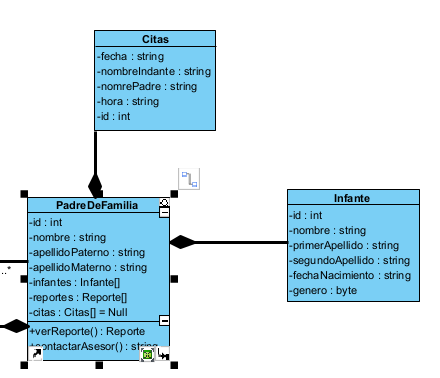
\includegraphics[width=0.4\textwidth]{images/arqui/colPadreFamilia.png}
\caption{Diagrama de la relacion del padre de familia con infantes.}
\label{fig:entidadpadin}
\end{figure}

\begin{figure}[htbp]
\centering
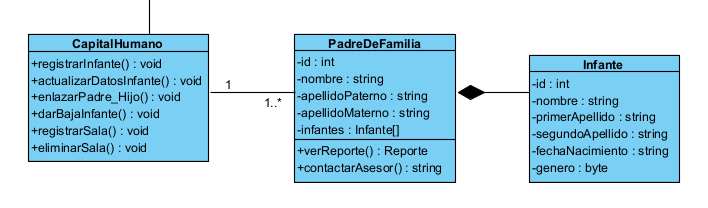
\includegraphics[width=0.4\textwidth]{images/arqui/capin.png}
\caption{Diagrama de la relacion de capital humano con padre e infantes.}
\label{fig:entidadpadin}
\end{figure}

\clearpage
%------------------------------------------------------------------
\subsection{Reporte}


\texttt{Reporte}, que representa un informe o registro de actividades y eventos relacionados con un infante en la guardería "Guardería Burbujas". Los reportes se utilizan para documentar diferentes aspectos del cuidado y el progreso del infante durante su estancia en la guardería.

La entidad \texttt{Reporte} tiene los siguientes atributos:

\begin{itemize}
\item \texttt{asistencia}: Registra la asistencia del infante a la guardería en un día específico.
\item \texttt{evacuaciones}: Registra las evacuaciones realizadas por el infante durante su estancia en la guardería, incluyendo información relevante como la frecuencia y características.
\item \texttt{ingesta}: Registra la información sobre la alimentación del infante, incluyendo la cantidad y tipo de alimentos consumidos.
\item \texttt{cambioRopa}: Registra los cambios de ropa realizados al infante, por ejemplo, en caso de accidentes o necesidades de higiene.
\item \texttt{informacionAdicional}: Permite registrar información adicional relevante sobre el infante, como observaciones especiales, necesidades particulares o eventos destacados.
\item \texttt{actividades}: Registra las actividades en las que el infante ha participado durante su jornada en la guardería, como juegos, ejercicios o tareas educativas.
\item \texttt{tareas}: Registra las tareas asignadas al infante para realizar en la guardería, como actividades de aprendizaje o responsabilidades específicas.
\item \texttt{nombreProfesor}: Almacena el nombre del profesor o encargado responsable de registrar el reporte del infante.
\end{itemize}


\begin{figure}[htbp]
\centering
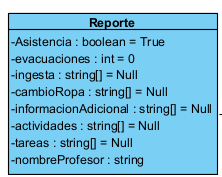
\includegraphics[width=0.4\textwidth]{images/arqui/Reporte.png}
\caption{Diagrama de la clase reporte.}
\label{fig:entidadreporte}
\end{figure}

\begin{figure}[htbp]
\centering
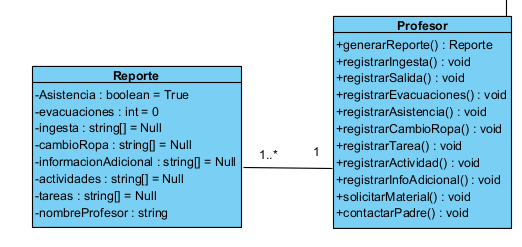
\includegraphics[width=0.4\textwidth]{images/arqui/reprof.png}
\caption{Diagrama de la relacion del profesor y los reportes.}
\label{fig:entidadpadre}
\end{figure}


\clearpage
%------------------------------------------------------------------
\subsection{Menu y comidas}


Esta entidad \texttt{Menú} y se compone de la entidad \texttt{Comida} es importante para planificar y organizar las comidas ofrecidas a los infantes.

La entidad \texttt{Menú} tiene los siguientes atributos:

\begin{itemize}
\item \texttt{id}: Identificador único del menú.
\item \texttt{comidas}: Una lista de comidas que conforman el menú. Cada comida está representada por un objeto de la entidad \texttt{Comida}.
\item \texttt{momentoDelDia}: Indica el momento del día al que corresponde el menú, como desayuno, almuerzo o merienda.
\item \texttt{kCalTotales}: El total de calorías estimadas para todas las comidas del menú.
\end{itemize}

La entidad \texttt{Comida} representa una comida específica que forma parte del menú. Tiene los siguientes atributos:

\begin{itemize}
\item \texttt{id}: Identificador único de la comida.
\item \texttt{nombre}: Nombre de la comida.
\item \texttt{ingredientes}: Lista de ingredientes utilizados en la preparación de la comida.
\item \texttt{kCal}: Cantidad de calorías estimadas para la comida.
\end{itemize}

La entidad \texttt{Menú} se compone de varias instancias de la entidad \texttt{Comida}, lo que permite definir y organizar las opciones de alimentación para los infantes en la guardería. Cada comida tiene su propio conjunto de atributos, como nombre, ingredientes y calorías, lo que facilita la planificación de las comidas de acuerdo con los requisitos nutricionales y las preferencias alimenticias.

La entidad \texttt{Menú y Comidas} es esencial en el contexto de la guardería, ya que garantiza que se ofrezcan opciones de alimentación equilibradas y adecuadas para los infantes, promoviendo su salud y bienestar. Además, permite mantener un registro de los alimentos servidos y proporcionar información relevante a los padres de familia y al personal encargado de la alimentación.



\begin{figure}[htbp]
\centering
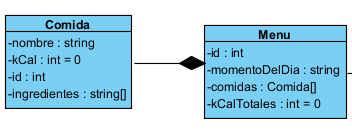
\includegraphics[width=0.4\textwidth]{images/arqui/menuComida.png}
\caption{Diagrama de la clase de Menu y de clase Comidas.}
\label{fig:entidamenucomida}
\end{figure}


\begin{figure}[htbp]
\centering
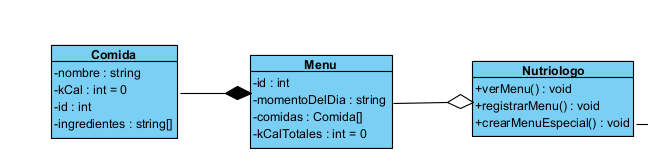
\includegraphics[width=0.4\textwidth]{images/arqui/comimennutr.png}
\caption{Diagrama de la relacion del menu con el nutriologo.}
\label{fig:entidamenucomida}
\end{figure}

\clearpage


%------------------------------------------------------------------
\subsection{Calendario y Eventos escolares.}

Para llevar un correcto manejo de los eventos escolares es que se usa un calendario, el cual se divide en dos entidades:
La entidad "Eventos Escolares" tiene los siguientes atributos:

\begin{itemize}
\item \textbf{ID:} Identificador único del evento escolar.
\item \textbf{Fecha:} Fecha en la que se llevará a cabo el evento escolar.
\item \textbf{Hora de Inicio:} Hora de inicio del evento escolar.
\item \textbf{Hora de Término:} Hora de término del evento escolar.
\item \textbf{Nombre:} Nombre o descripción del evento escolar.
\end{itemize}

La entidad "Calendario" tiene los siguientes atributos:

\begin{itemize}
\item \textbf{ID:} Identificador único del calendario.
\item \textbf{Eventos Escolares:} Un arreglo que almacena los eventos escolares programados en el calendario.
\end{itemize}


\begin{figure}[htbp]
\centering
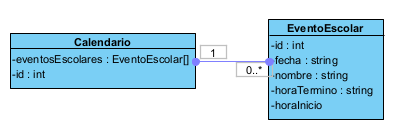
\includegraphics[width=0.4\textwidth]{images/arqui/colCaEv.png}
\caption{Diagrama de la relacion Eventos Escolares con calendario}
\label{fig:colecEventCald}
\end{figure}

\clearpage


%------------------------------------------------------------------
\subsection{Salas.}

Las Salas son nuestras Salas en la guarderia, es por eso que es indispensable llevar un control de estas con su identificador y numero de capacidad.
La entidad "Sala" tiene los siguientes atributos:

\begin{itemize}
\item \textbf{ID:} Identificador único del evento escolar.
\item \textbf{Capacidad:} La capacidad maxima de esa sala
\end{itemize}


\begin{figure}[htbp]
\centering
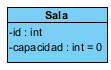
\includegraphics[width=0.4\textwidth]{images/arqui/sala.png}
\caption{Diagrama de la entidad sala}
\label{fig:colecSala}
\end{figure}
\clearpage